% =========================================================
% Section: Mechanism -- Limited Direct Execution
% =========================================================

\section{Direct Execution}

% ---------------------------------------------------------
\begin{frame}{CPU Virtualization: The Main Challenge}

\begin{block}{Goal}
The operating system must virtualize the CPU efficiently
while retaining control over the system.
\end{block}

\begin{itemize}
    \item The CPU is shared among multiple processes through
          \textbf{time sharing}.
    \item Two central challenges:
    \begin{itemize}
        \item \textbf{Performance}: minimize virtualization overhead.
        \item \textbf{Control}: prevent processes from taking over the system.
    \end{itemize}
    \item Hardware and operating-system support are both required.
\end{itemize}

\end{frame}

% ---------------------------------------------------------
\begin{frame}{Basic Technique (Mechanism): Limited Direct Execution}

\begin{itemize}
    \item The basic idea is to run programs \textbf{directly on the CPU}.
    \item Direct execution provides high performance.
    \item Before execution, the OS:
    \begin{itemize}
        \item creates a process entry;
        \item allocates memory;
        \item loads the program;
        \item prepares the stack;
        \item starts execution at the program entry point.
    \end{itemize}
\end{itemize}

\begin{alertblock}{Problem}
How can the OS run a program directly while still maintaining
control over the CPU?
\end{alertblock}

\end{frame}

% ---------------------------------------------------------
\begin{frame}{Direct Execution Without Limits}

\begin{columns}[T]
    \begin{column}{0.45\textwidth}
        \begin{itemize}
            \item The OS starts the program.
            \item The program executes directly on the processor.
            \item When it finishes, control returns to the OS.
        \end{itemize}

        \vspace{0.2cm}

        Two problems emerge:
        \begin{enumerate}
            \item How to restrict privileged operations?
            \item How to regain control of the CPU?
        \end{enumerate}
    \end{column}

    \begin{column}{0.52\textwidth}
    \begin{figure}
        \centering
        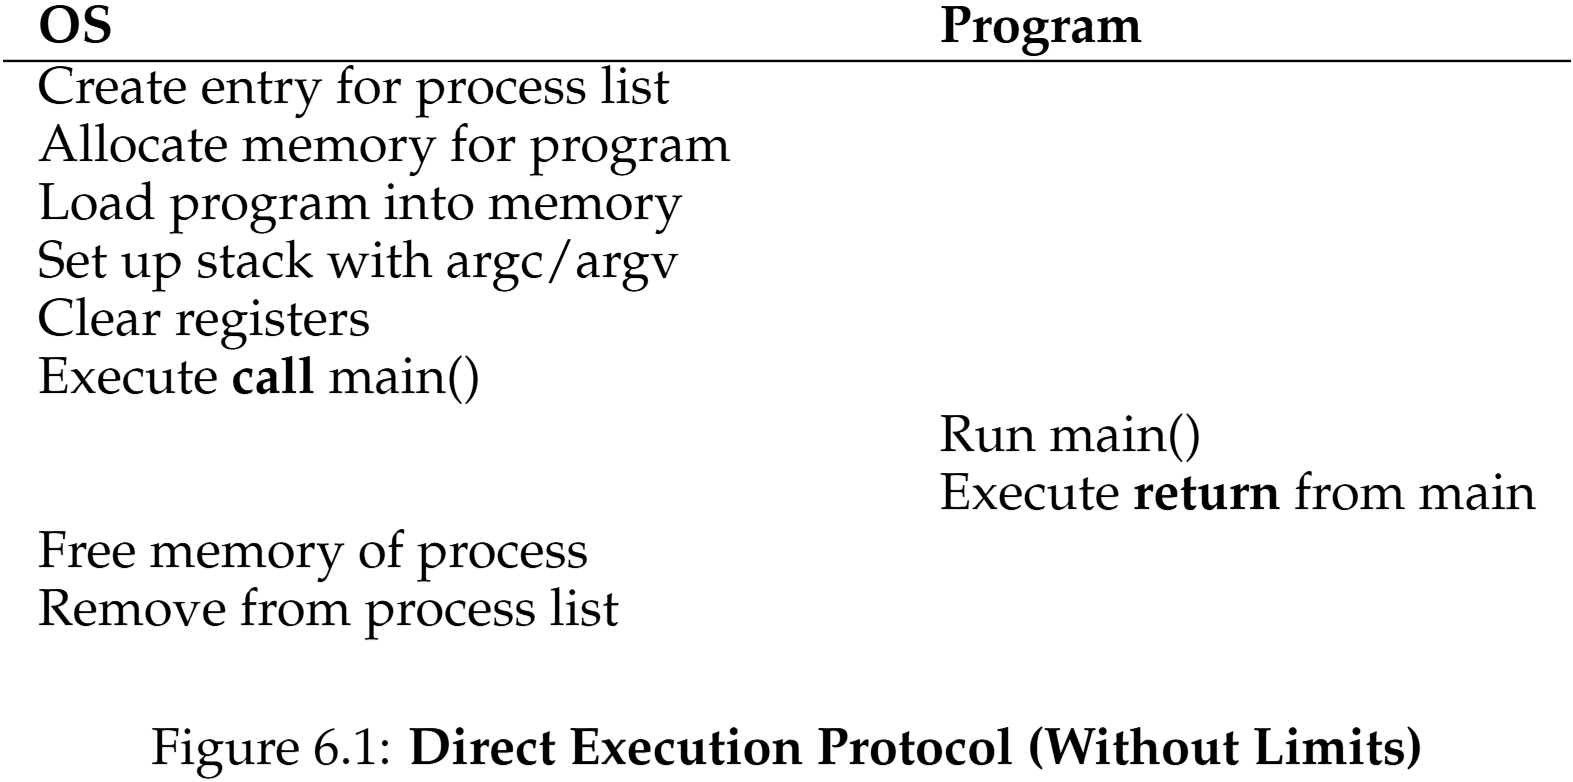
\includegraphics[width=1.1\linewidth]{figs/chapter-6/figure-6.1.png}
        \caption*{Source: chapter page 2.}
        \label{fig:figure-6.1}
    \end{figure}
    \end{column}
\end{columns}

\end{frame}

% ---------------------------------------------------------
\subsection*{Restricted Operations}

\begin{frame}{Problem \#1: Restricted Operations}

\begin{block}{The Crux}
A process must perform I/O and other restricted operations
without gaining complete control over the system.
\end{block}

\begin{itemize}
    \item Direct execution alone would allow applications to perform
          operations that should be controlled by the OS.
    \item The processor therefore supports different execution modes:
    \begin{itemize}
        \item \textbf{User mode}: restricted execution.
        \item \textbf{Kernel mode}: privileged execution.
    \end{itemize}
    \item Privileged operations are performed by the operating system.
\end{itemize}

\end{frame}

% ---------------------------------------------------------
\begin{frame}{System Calls and Protected Control Transfer}

\begin{itemize}
    \item User programs request OS services through
          \textbf{system calls}.
    \item A system call uses a special \textbf{trap instruction}.
    \item The trap:
    \begin{enumerate}
        \item saves the required processor state;
        \item switches execution to kernel mode;
        \item transfers control to a predefined OS handler.
    \end{enumerate}
    \item The OS performs the requested operation.
    \item A \textbf{return-from-trap} instruction restores execution
          in user mode.
\end{itemize}

\begin{block}{Key Idea}
System calls provide controlled access to privileged OS services.
\end{block}

\end{frame}

% ---------------------------------------------------------
\begin{frame}{Why System Calls Look Like Procedure Calls}

\begin{itemize}
    \item Calls such as \texttt{open()} and \texttt{read()} appear
          to be ordinary C procedure calls.
    \item The C library prepares:
    \begin{itemize}
        \item system-call arguments;
        \item the system-call number.
    \end{itemize}
    \item Library code then executes the hardware-specific
          \textbf{trap instruction}.
    \item After returning from the kernel, the library processes the
          return value and returns control to the application.
\end{itemize}

\end{frame}

% ---------------------------------------------------------
\begin{frame}{The Trap Table}

\begin{itemize}
    \item User programs cannot choose arbitrary kernel addresses
          as trap destinations.
    \item During boot, the OS initializes a \textbf{trap table}.
    \item The table defines handlers for events such as:
    \begin{itemize}
        \item system calls;
        \item hardware interrupts;
        \item exceptional conditions.
    \end{itemize}
    \item Installing the trap table is a
          \textbf{privileged operation}.
\end{itemize}

\begin{alertblock}{Protection}
User code requests a service through a system-call number,
rather than specifying an arbitrary kernel address.
\end{alertblock}

\end{frame}

% ---------------------------------------------------------
\begin{frame}{Limited Direct Execution Protocol}

\centering

\begin{figure}
    \centering
    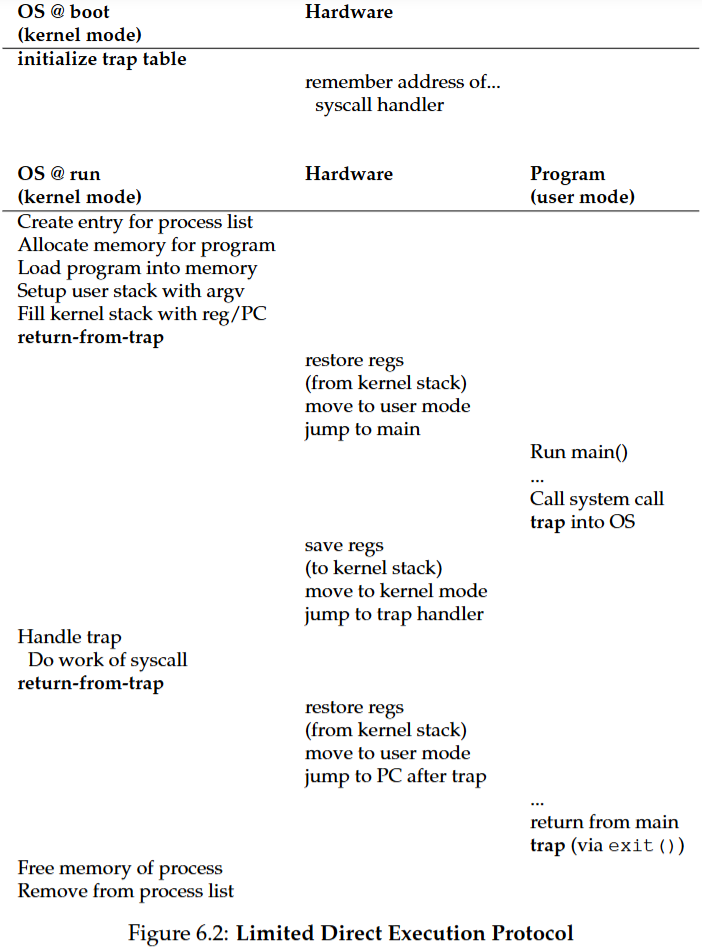
\includegraphics[width=0.5\linewidth]{figs/chapter-6/figure-6.2.png}
    \caption*{Source: chapter page 5.}
    \label{fig:figure-6.2}
\end{figure}

\end{frame}

% ---------------------------------------------------------
\subsection*{Regaining Control of the CPU}

\begin{frame}{Problem \#2: Switching Between Processes}

\begin{block}{The Crux}
How can the operating system regain control of the CPU
while a process is running?
\end{block}

\begin{itemize}
    \item If a user process is executing, the OS itself is not executing.
    \item The OS therefore needs a mechanism to regain control.
    \item Two approaches are discussed:
    \begin{itemize}
        \item cooperative;
        \item non-cooperative.
    \end{itemize}
\end{itemize}

\end{frame}

% ---------------------------------------------------------
\begin{frame}{Cooperative Approach}

\begin{itemize}
    \item The OS waits for the process to voluntarily transfer control.
    \item Control can return to the OS through:
    \begin{itemize}
        \item system calls;
        \item an explicit \texttt{yield()} system call;
        \item traps caused by illegal operations.
    \end{itemize}
\end{itemize}

\begin{alertblock}{Limitation}
A process running forever without making a system call
could monopolize the CPU.
\end{alertblock}

\end{frame}

% ---------------------------------------------------------
\begin{frame}{Non-Cooperative Approach: Timer Interrupt}

\begin{itemize}
    \item Hardware provides a programmable
          \textbf{timer interrupt}.
    \item The timer periodically interrupts the running process.
    \item When the interrupt occurs:
    \begin{enumerate}
        \item the running process is halted;
        \item its state is saved;
        \item the CPU switches to kernel mode;
        \item the OS interrupt handler executes.
    \end{enumerate}
    \item The OS has regained control of the CPU.
\end{itemize}

\begin{block}{Key Mechanism}
The timer interrupt prevents a process from monopolizing the CPU.
\end{block}

\end{frame}

% ---------------------------------------------------------
\subsection*{Context Switching}

\begin{frame}{Saving and Restoring Context}

\begin{itemize}
    \item After regaining control, the OS scheduler decides whether:
    \begin{itemize}
        \item to continue executing the current process; or
        \item to switch to another process.
    \end{itemize}

    \item A \textbf{context switch} saves the state of one process
          and restores the state of another.

    \item Relevant state includes:
    \begin{itemize}
        \item general-purpose registers;
        \item program counter;
        \item kernel stack pointer.
    \end{itemize}
\end{itemize}

\end{frame}

% ---------------------------------------------------------
\begin{frame}{Timer Interrupt and Context Switch}

\begin{columns}[T]
    \begin{column}{0.38\textwidth}
        \begin{itemize}
            \item Process A is executing.
            \item A timer interrupt occurs.
            \item Hardware saves A's user state.
            \item The OS enters the interrupt handler.
            \item The OS switches from A to B.
            \item B resumes execution.
        \end{itemize}
    \end{column}

    \begin{column}{0.60\textwidth}
    \begin{figure}
        \centering
        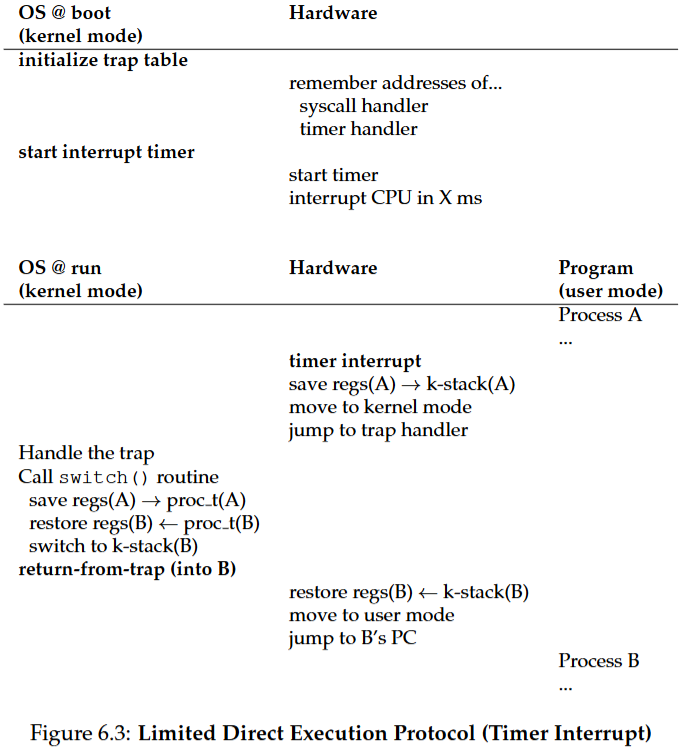
\includegraphics[width=0.9\linewidth]{figs/chapter-6/figure-6.3.png}
        \caption*{Source: chapter page 11.}
        \label{fig:figure-6.3}
    \end{figure}
    \end{column}
\end{columns}

\end{frame}

% ---------------------------------------------------------
\begin{frame}{Two Types of State Saving}

\begin{enumerate}
    \item \textbf{Hardware save/restore}
    \begin{itemize}
        \item occurs when the timer interrupt happens;
        \item saves the user registers;
        \item uses the process kernel stack.
    \end{itemize}

    \vspace{0.3cm}

    \item \textbf{Software save/restore}
    \begin{itemize}
        \item occurs during the context switch;
        \item performed explicitly by the OS;
        \item saves and restores kernel context.
    \end{itemize}
\end{enumerate}

\end{frame}

% ---------------------------------------------------------
\begin{frame}{Example: xv6 Context Switch}

\begin{columns}[T]
    \begin{column}{0.35\textwidth}
        \begin{itemize}
            \item Save registers of the old process.
            \item Restore registers of the new process.
            \item Switch the kernel stack.
            \item Return into the new execution context.
        \end{itemize}
    \end{column}

    \begin{column}{0.63\textwidth}
    \begin{figure}
        \centering
        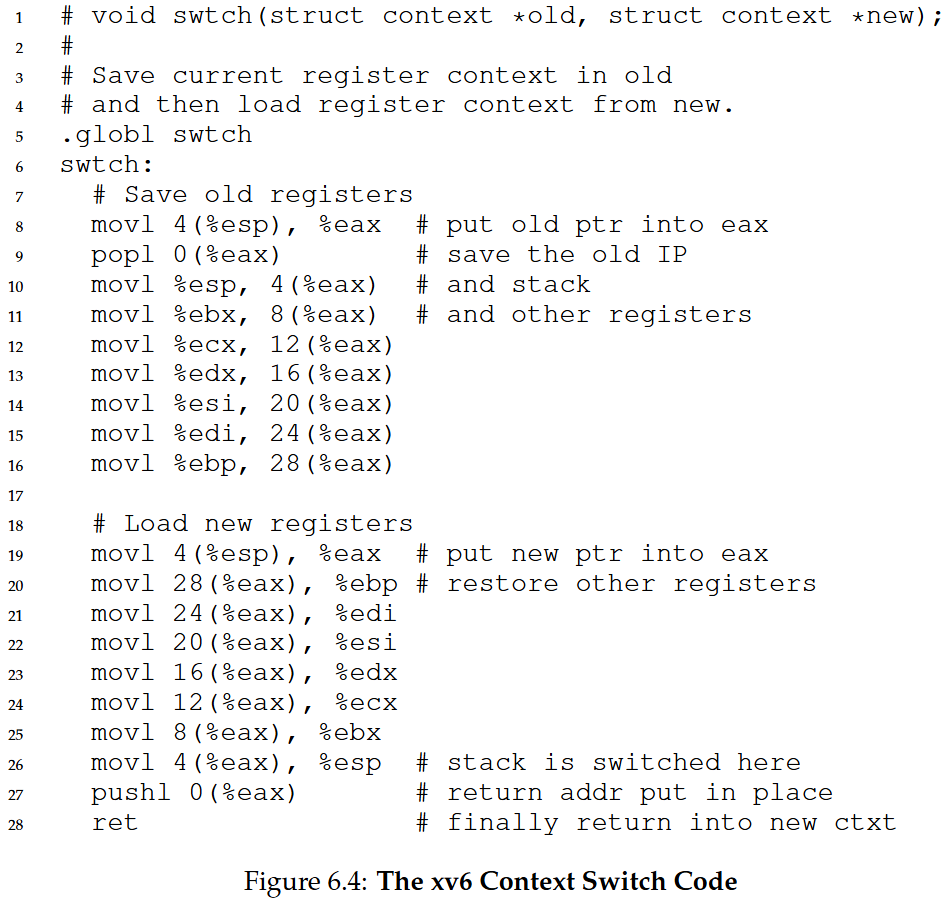
\includegraphics[width=1.1\linewidth]{figs/chapter-6/figure-6.4.png}
        \caption*{Source: chapter page 12.}
        \label{fig:figure-6.4}
    \end{figure}
    \end{column}
\end{columns}

\end{frame}

% ---------------------------------------------------------
\subsection*{Concurrency}

\begin{frame}{What About Concurrency?}

\begin{itemize}
    \item What happens if a timer interrupt occurs during a system call?
    \item What happens if another interrupt arrives while one is being handled?
\end{itemize}

\vspace{0.3cm}

The chapter briefly introduces two approaches:

\begin{itemize}
    \item temporarily disabling interrupts during interrupt processing;
    \item using locking mechanisms to protect kernel data structures.
\end{itemize}

\begin{block}{Next Step}
Detailed treatment of these problems belongs to the study of
\textbf{concurrency}.
\end{block}

\end{frame}

% ---------------------------------------------------------
\begin{frame}{Limited Direct Execution: Summary}

\begin{itemize}
    \item Programs execute directly on the CPU for high performance.
    \item \textbf{User mode} restricts application privileges.
    \item \textbf{Kernel mode} allows privileged operations.
    \item \textbf{System calls} use traps to enter the kernel safely.
    \item A \textbf{trap table} determines valid kernel entry points.
    \item A \textbf{timer interrupt} allows the OS to regain CPU control.
    \item A \textbf{context switch} changes the running process.
\end{itemize}

\begin{block}{Central Idea}
Limited direct execution combines efficient execution with
operating-system control.
\end{block}

\end{frame}

% ---------------------------------------------------------
\begin{frame}{Performance Measurement}

The chapter suggests measuring two fundamental operating-system costs:

\begin{itemize}
    \item \textbf{System-call cost}
    \begin{itemize}
        \item repeatedly execute a simple system call;
        \item measure total execution time;
        \item estimate the average cost per call.
    \end{itemize}

    \item \textbf{Context-switch cost}
    \begin{itemize}
        \item use two processes communicating through UNIX pipes;
        \item force repeated switches between the processes;
        \item measure the communication cycle.
    \end{itemize}
\end{itemize}

\begin{block}{Tools Mentioned in the Chapter}
\texttt{gettimeofday()}, \texttt{rdtsc}, \texttt{sched\_setaffinity()},
and \texttt{lmbench}.
\end{block}

\end{frame}

\begin{frame}{Direct Execution: Summary}

\begin{itemize}
    \item \textbf{Limited Direct Execution} combines performance and OS control.
    \item \textbf{User/kernel modes} restrict privileged operations.
    \item \textbf{System calls} use traps to safely enter the kernel.
    \item \textbf{Timer interrupts} allow the OS to regain CPU control.
    \item \textbf{Context switches} enable execution to move between processes.
\end{itemize}

\vspace{0.4cm}

\begin{block}{Next Step}
With these mechanisms in place, the remaining question is:

\begin{center}
\textbf{Which process should run at a given time?}
\end{center}

This is the responsibility of the \textbf{CPU scheduler}.
\end{block}

\end{frame}